\chapter{Implementazione}

\section{Scheduler}
Come prima osservazione specifichiamo che la classe \texttt{RMScheduler} è una sotto classe di \texttt{Scheduler}. questo permette in futuro di implementare altri tipi di scheduler e di dataarli facilmente al sistema.

Ogni oggetto che estende \texttt{Scheduler} ha, oltre a ciò che definisce uno scheduler (e.g. taskSet e l'eventuale protocollo di accesso alle risorse), un oggetto di tipo \texttt{MyClock} che rappresenta il clock globale del sistema e una lista di task bloccati \texttt{blockedTask}.

Ogni scheduler deve associare una priorità; ad esempio RM la assegna in modo opposto rispetto alla durata del periodo. Questo compito è delegato dal metodo \texttt{assignPriority}. Ovviamente poi abbiamo il metodo \texttt{schedule} che viene chiamato per avviare la simulazione.

\subsection{Rate Monotonic}
Descriviamo brevemente l'idea di implementazione di RM e osserviamo il relativo Sequence Diagram in Figura \ref{fig:sdRM}.

Durante la creazione dello scheduler si fa un controllo per valutare che tutti i task del taskSet siano puramente periodici.

\begin{figure}[htbp]
    \centering
    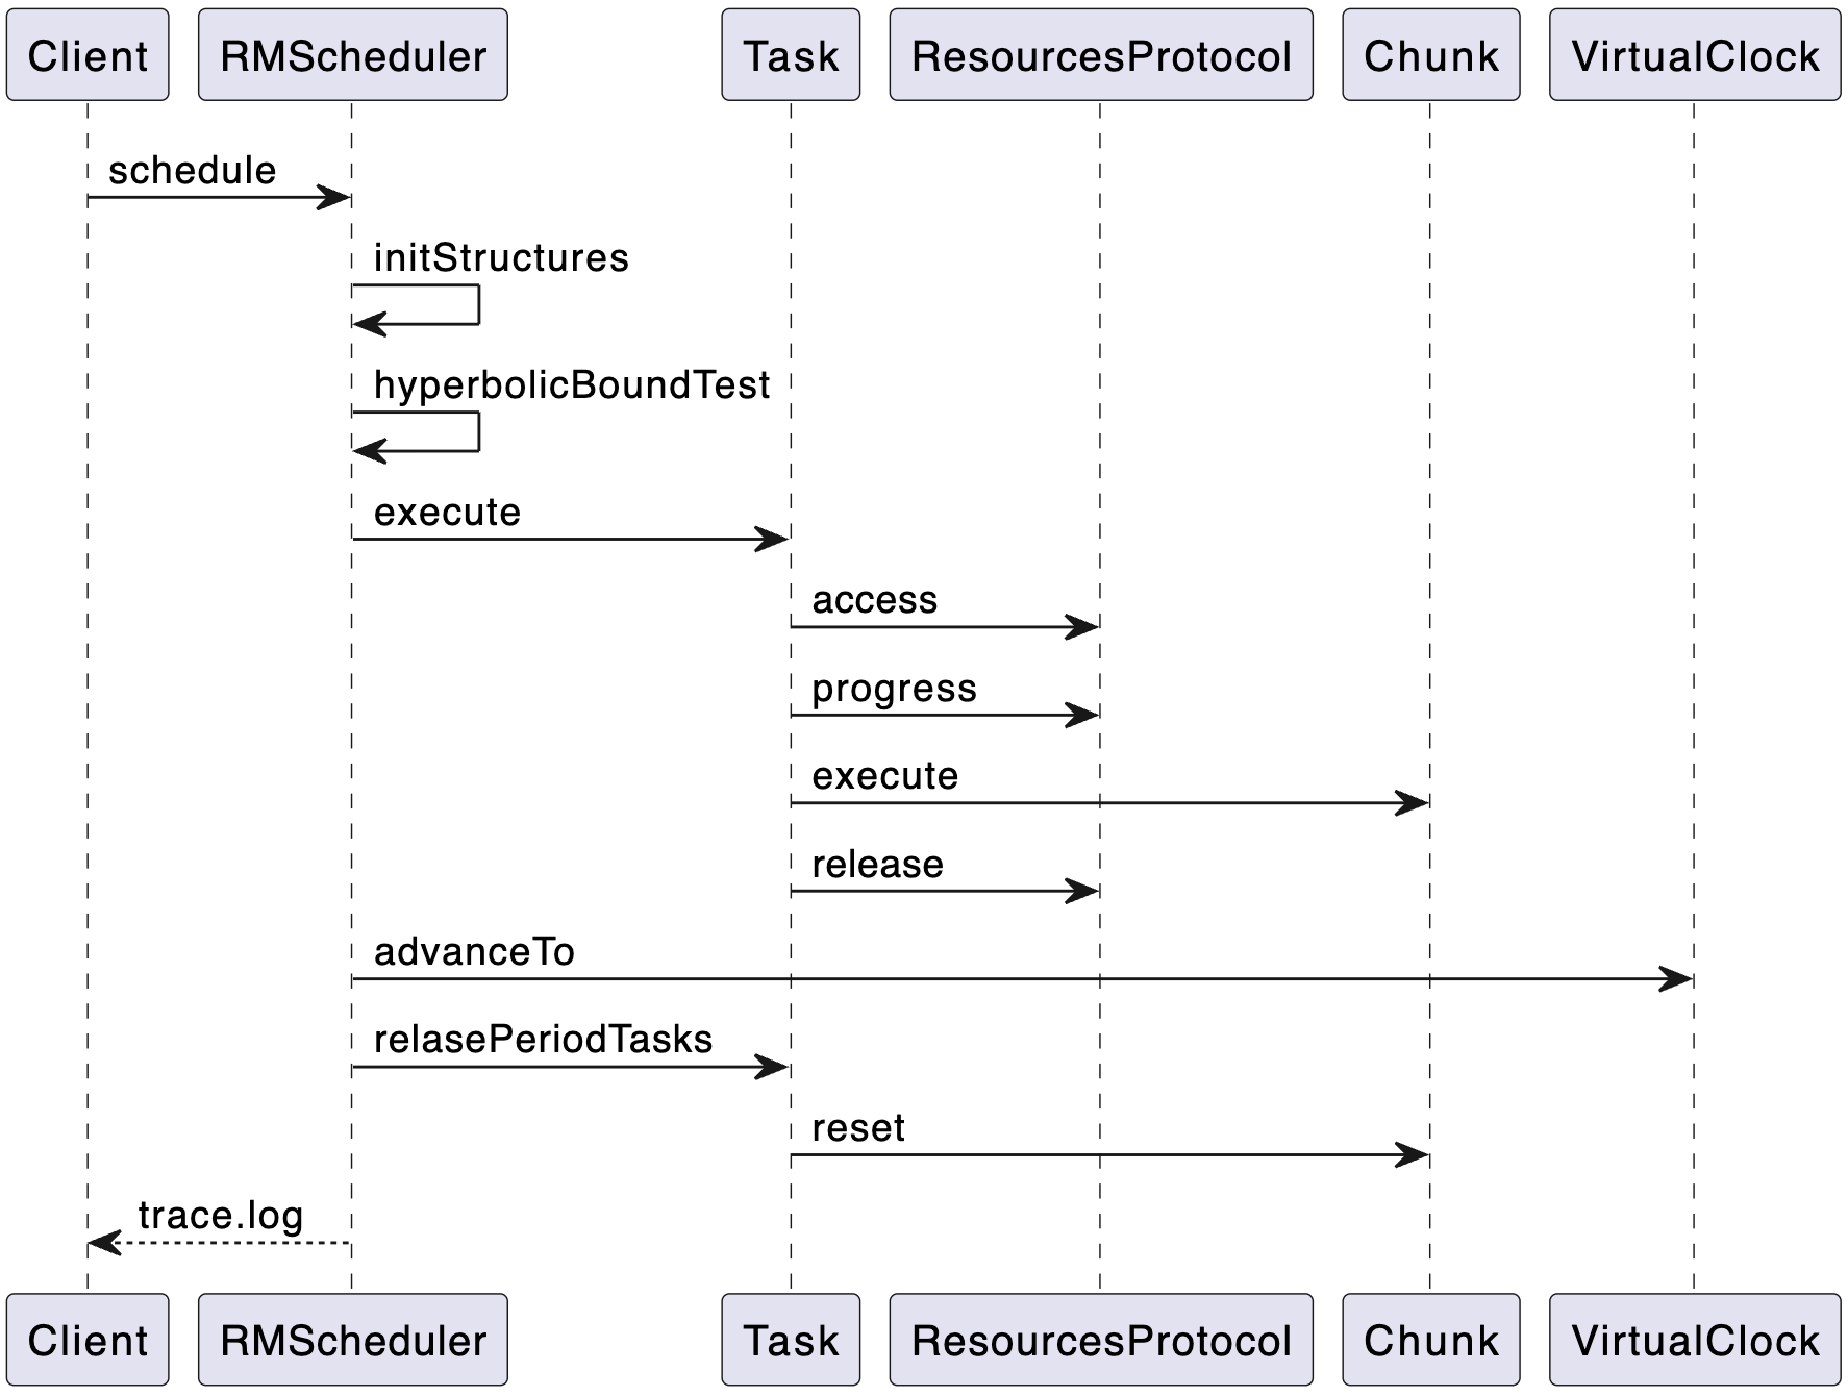
\includegraphics[width=1\textwidth]{immagini/sequence diagram RM.pdf}
    \caption{Sequence Siagram RM}
    \label{fig:sdRM}
\end{figure}

\myskip

La simulazione si basa su due strutture principali:
\begin{itemize}
    \item \texttt{taskReady} \\
        Ospita i task che si contendono l'accesso alla CPU. Al suo interno si usa un'ordinamento inverso rispetto alla durata del periodo dei vari task.
    \item \texttt{events} \\
        Gestisce gli eventi importnati, cioè i momenti in cui finisce il periodo di un task. Nell'intervallo tra un perido e il successivo infatti lo scheduler non fa altro che mandare in esecuzione uno dopo l'altro il task a priorità maggiore. Quando arriva il momento di un evento, vengono controllati i task il cui periodo è finito; questo controllo serve per valutare se una deadline è stata mancata e per rilasciare nuovamente il task nel caso non ci siano errori. Gli eventi sono l’unione ordinata dei multipli di ciascun periodo fino al minimo comune multiplo dei periodi oppure fino a 10 volte il periodo maggiore (per semplicità del caso sia molto oneroso gestire questa lista).
\end{itemize}

\myskip

Il metodo \texttt{schedule} poi delega la gestione dei chunk di ogni task alla classe \texttt{Task}, la quale a sua volta rimanda alla calsse \texttt{Chunk} la loro esecuione (e.g. il logging).

\section{Resource Access Protocol}
Ogni implementazione di un protocollo di accesso alle risorse deve estendere la classe \texttt{ResourceProtocol}.

I metodi definiti da questa classe astratta sono le operazioni che devono essere svolte da un procotollo di questo tipo: deve gestire la fase di accesso, progresso e rilascio. Definisce anche il metodo \texttt{initStructures} che ha il compito di inizializzare le strutture dati usate dal protocollo.

\subsection{Priority Ceiling Protocol}
Tralasciando quello che fanno i metodi di accesso, progresso e rilascio, che riflettono quanto ci dice la teoria, in questo classe le strutture usate sono prevalentemente due:
\begin{itemize}
    \item \texttt{ceiling} \\
        È una mappa che associata ad ogni risorsa il suo ceiling, cioè la massima priorità nominale dei task che usano quella risorsa.
    \item \texttt{busyResources}\\
        È una losta delle risorse che sono occupate da un qualche task.
\end{itemize}

\section{Utilità}
In questo capitolo sono brevemente descritte le scelte di alcuni componenti di utilità.

\subsection{Loggin}
Per il logging è stato implementato un semplice logging su un file e viene rappresnetato come una sequenza di coppie $<evento,tempo>$.

Il file di destinazione delle tracce loggate è \texttt{trace.log}.

\subsection{Clock}
Il clock del sistema è rappresnetato dalla classe \texttt{MyClock}. Questa non fa altro che mantenere il tempo assoluto ed esporre due metodi che permettono di avanzare di un dato intervallo temporale e avanzare fino a un determinato tempo.

Il tempo è gestito tramite oggetti di tipo \texttt{Duration}, che implementa oggetti immutabili e che permetto una facile gestione del tempo.

\subsection{Sampling dei tempi}
Quando si deve definire i tempi che definiscono i vari componenti del sistema, cioè come il periodo, la dealine, l'execution time di un chunk, si usa un campionamento da un data distribuzione.

Le distribuzioni sono data dalla libreria \texttt{Sirio}; oltre a quelle definite dalla libreria è stata implementata la classe \texttt{ConstantSampler}, che permette di gestire tempi costanti, mantenendo l'astrazione della libreria Sirio.